\documentclass{beamer}

% xcolor and define colors -------------------------
\usepackage{xcolor}

% https://www.viget.com/articles/color-contrast/
\definecolor{purple}{HTML}{5601A4}
\definecolor{navy}{HTML}{0D3D56}
\definecolor{ruby}{HTML}{9a2515}
\definecolor{alice}{HTML}{107895}
\definecolor{daisy}{HTML}{EBC944}
\definecolor{coral}{HTML}{F26D21}
\definecolor{kelly}{HTML}{829356}
\definecolor{cranberry}{HTML}{E64173}
\definecolor{jet}{HTML}{131516}
\definecolor{asher}{HTML}{555F61}
\definecolor{slate}{HTML}{314F4F}

% Mixtape Sessions
\definecolor{picton-blue}{HTML}{00b7ff}
\definecolor{violet-red}{HTML}{ff3881}
\definecolor{sun}{HTML}{ffaf18}
\definecolor{electric-violet}{HTML}{871EFF}

% Main theme colors
\definecolor{accent}{HTML}{00b7ff}
\definecolor{accent2}{HTML}{871EFF}
\definecolor{gray100}{HTML}{f3f4f6}
\definecolor{gray800}{HTML}{1F292D}


% Beamer Options -------------------------------------

% Background
\setbeamercolor{background canvas}{bg = white}

% Change text margins
\setbeamersize{text margin left = 15pt, text margin right = 15pt} 

% \alert
\setbeamercolor{alerted text}{fg = accent2}

% Frame title
\setbeamercolor{frametitle}{bg = white, fg = jet}
\setbeamercolor{framesubtitle}{bg = white, fg = accent}
\setbeamerfont{framesubtitle}{size = \small, shape = \itshape}

% Block
\setbeamercolor{block title}{fg = white, bg = accent2}
\setbeamercolor{block body}{fg = gray800, bg = gray100}

% Title page
\setbeamercolor{title}{fg = gray800}
\setbeamercolor{subtitle}{fg = accent}

%% Custom \maketitle and \titlepage
\setbeamertemplate{title page}
{
    %\begin{centering}
        \vspace{20mm}
        {\Large \usebeamerfont{title}\usebeamercolor[fg]{title}\inserttitle}\\
        {\large \itshape \usebeamerfont{subtitle}\usebeamercolor[fg]{subtitle}\insertsubtitle}\\ \vspace{10mm}
        {\insertauthor}\\
        {\color{asher}\small{\insertdate}}\\
    %\end{centering}
}

% Table of Contents
\setbeamercolor{section in toc}{fg = accent!70!jet}
\setbeamercolor{subsection in toc}{fg = jet}

% Button 
\setbeamercolor{button}{bg = accent}

% Remove navigation symbols
\setbeamertemplate{navigation symbols}{}

% Table and Figure captions
\setbeamercolor{caption}{fg=jet!70!white}
\setbeamercolor{caption name}{fg=jet}
\setbeamerfont{caption name}{shape = \itshape}

% Bullet points

%% Fix left-margins
\settowidth{\leftmargini}{\usebeamertemplate{itemize item}}
\addtolength{\leftmargini}{\labelsep}

%% enumerate item color
\setbeamercolor{enumerate item}{fg = accent}
\setbeamerfont{enumerate item}{size = \small}
\setbeamertemplate{enumerate item}{\insertenumlabel.}

%% itemize
\setbeamercolor{itemize item}{fg = accent!70!white}
\setbeamerfont{itemize item}{size = \small}
\setbeamertemplate{itemize item}[circle]

%% right arrow for subitems
\setbeamercolor{itemize subitem}{fg = accent!60!white}
\setbeamerfont{itemize subitem}{size = \small}
\setbeamertemplate{itemize subitem}{$\rightarrow$}

\setbeamertemplate{itemize subsubitem}[square]
\setbeamercolor{itemize subsubitem}{fg = jet}
\setbeamerfont{itemize subsubitem}{size = \small}







% Links ----------------------------------------------

\usepackage{hyperref}
\hypersetup{
  colorlinks = true,
  linkcolor = accent2,
  filecolor = accent2,
  urlcolor = accent2,
  citecolor = accent2,
}


% Line spacing --------------------------------------
\usepackage{setspace}
\setstretch{1.1}


% \begin{columns} -----------------------------------
\usepackage{multicol}


% Fonts ---------------------------------------------
% Beamer Option to use custom fonts
\usefonttheme{professionalfonts}

% \usepackage[utopia, smallerops, varg]{newtxmath}
% \usepackage{utopia}
\usepackage[sfdefault,light]{roboto}

% Small adjustments to text kerning
\usepackage{microtype}



% Remove annoying over-full box warnings -----------
\vfuzz2pt 
\hfuzz2pt


% Table of Contents with Sections
\setbeamerfont{myTOC}{series=\bfseries, size=\Large}
\AtBeginSection[]{
        \frame{
            \frametitle{Roadmap}
            \tableofcontents[current]   
        }
    }


% Tables -------------------------------------------
% Tables too big
% \begin{adjustbox}{width = 1.2\textwidth, center}
\usepackage{adjustbox}
\usepackage{array}
\usepackage{threeparttable, booktabs, adjustbox}
    
% Fix \input with tables
% \input fails when \\ is at end of external .tex file
\makeatletter
\let\input\@@input
\makeatother

% Tables too narrow
% \begin{tabularx}{\linewidth}{cols}
% col-types: X - center, L - left, R -right
% Relative scale: >{\hsize=.8\hsize}X/L/R
\usepackage{tabularx}
\newcolumntype{L}{>{\raggedright\arraybackslash}X}
\newcolumntype{R}{>{\raggedleft\arraybackslash}X}
\newcolumntype{C}{>{\centering\arraybackslash}X}

% Figures

% \imageframe{img_name} -----------------------------
% from https://github.com/mattjetwell/cousteau
\newcommand{\imageframe}[1]{%
    \begin{frame}[plain]
        \begin{tikzpicture}[remember picture, overlay]
            \node[at = (current page.center), xshift = 0cm] (cover) {%
                \includegraphics[keepaspectratio, width=\paperwidth, height=\paperheight]{#1}
            };
        \end{tikzpicture}
    \end{frame}%
}

% subfigures
\usepackage{subfigure}


% Highlight slide -----------------------------------
% \begin{transitionframe} Text \end{transitionframe}
% from paulgp's beamer tips
\newenvironment{transitionframe}{
    \setbeamercolor{background canvas}{bg=accent!40!black}
    \begin{frame}\color{accent!10!white}\LARGE\centering
}{
    \end{frame}
}


% Table Highlighting --------------------------------
% Create top-left and bottom-right markets in tabular cells with a unique matching id and these commands will outline those cells
\usepackage[beamer,customcolors]{hf-tikz}
\usetikzlibrary{calc}
\usetikzlibrary{fit,shapes.misc}

% To set the hypothesis highlighting boxes red.
\newcommand\marktopleft[1]{%
    \tikz[overlay,remember picture] 
        \node (marker-#1-a) at (0,1.5ex) {};%
}
\newcommand\markbottomright[1]{%
    \tikz[overlay,remember picture] 
        \node (marker-#1-b) at (0,0) {};%
    \tikz[accent!80!jet, ultra thick, overlay, remember picture, inner sep=4pt]
        \node[draw, rectangle, fit=(marker-#1-a.center) (marker-#1-b.center)] {};%
}

\usepackage{breqn} % Breaks lines

\usepackage{amsmath}
\usepackage{mathtools}

\usepackage{pdfpages} % \includepdf

\usepackage{listings} % R code
\usepackage{verbatim} % verbatim

% Video stuff
\usepackage{media9}

% packages for bibs and cites
\usepackage{natbib}
\usepackage{har2nat}
\newcommand{\possessivecite}[1]{\citeauthor{#1}'s \citeyearpar{#1}}
\usepackage{breakcites}
\usepackage{alltt}

% Setup math operators
\DeclareMathOperator{\E}{E} \DeclareMathOperator{\tr}{tr} \DeclareMathOperator{\se}{se} \DeclareMathOperator{\I}{I} \DeclareMathOperator{\sign}{sign} \DeclareMathOperator{\supp}{supp} \DeclareMathOperator{\plim}{plim}
\DeclareMathOperator*{\dlim}{\mathnormal{d}\mkern2mu-lim}
\newcommand\independent{\protect\mathpalette{\protect\independenT}{\perp}}
   \def\independenT#1#2{\mathrel{\rlap{$#1#2$}\mkern2mu{#1#2}}}
\newcommand*\colvec[1]{\begin{pmatrix}#1\end{pmatrix}}

\newcommand{\myurlshort}[2]{\href{#1}{\textcolor{gray}{\textsf{#2}}}}


\begin{document}

\imageframe{./lecture_includes/mixtape_did_cover.png}


% ---- Content ----

\section{Introduction}

\subsection{Managing expectations}


\begin{frame}{Introduction}

\begin{itemize}
\item Welcome to Mixtape Sessions workshop on difference-in-differences and synthetic control (``Causal Inference II'')
\item 8:00am to 5:00pm CST, 15 min breaks every hour, 1 hour lunch at noon CST
\item Lecture, discussion, exercises, application
\end{itemize}

\end{frame}


\begin{frame}{Workshop outline}

Introduction to DiD basics 
	\begin{itemize}
	\item Potential outcomes review
	\item DiD equation and estimation with OLS
	\item Evaluating parallel trends with falsifications, event studies 
	\item Triple differences
	\item Including covariates
	\end{itemize}

\end{frame}


\begin{frame}{Workshop outline}

 Differential timing
	\begin{itemize}
	\item Bacon decomposition 
	\item Aggregating group-time ATTs
	\item Issues and solutions with event studies
	\item Turning treatments on and off
	\item Stacked regression
	\item Imputation estimators
	\item Continuous treatments
	\end{itemize}

\end{frame}

\begin{frame}{Workshop outline}

Synthetic control

\begin{itemize}
\item Canonical synth
\end{itemize}

\end{frame}

\subsection{Introducing difference-in-differences}

\imageframe{./lecture_includes/bumpersticker.jpeg}


\begin{frame}{Natural experiments}

\begin{quote}
``A good way to do econometrics is to look for good natural experiments and use statistical methods that can tidy up the confounding factors that nature has not controlled for us.'' -- Daniel McFadden (Nobel Laureate recipient with Heckman 1992)
\end{quote}

\end{frame}




\begin{frame}{What is difference-in-differences (DiD)}

\begin{itemize}
\item DiD is a very old, relatively straightforward, intuitive research design
\item A group of units are assigned some treatment and then compared to a group of units that weren't
\item One of the most widely used quasi-experimental methods in economics and even used in industry
\item Mostly associated with ``big shocks'' happening in space over time
\end{itemize}

\end{frame}


\begin{frame}

	\begin{figure}
	\caption{Currie, et al. (2020)}
	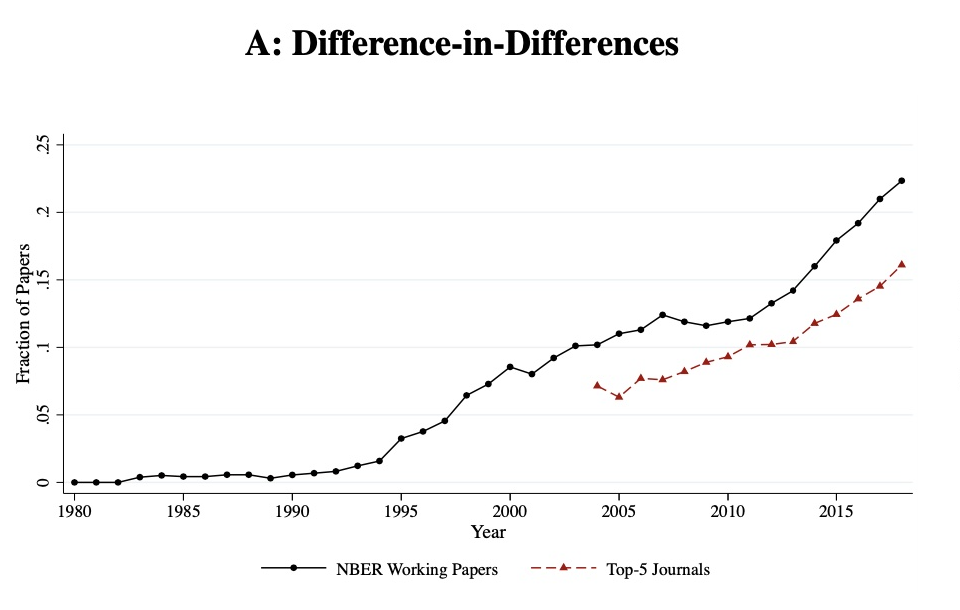
\includegraphics[scale=0.25]{./lecture_includes/currie_did.png}
	\end{figure}


\end{frame}






\begin{frame}{Why an entire workshop on DiD?}

\begin{itemize}
\item \textbf{Research advantages}: DiD is sometimes the only way we have to study large social policies 
\item \textbf{Good time to retool}: Recent wave of scholarship suggest model misspecification is pronounced
\item \textbf{Good news}: Better understanding of our models, new tools, new programs
\item \textbf{Hope}: I think we can get to the bottom of this in a way that will stick with you
\end{itemize}

\end{frame}











\subsection{History}

\begin{frame}{Brief history of diff-in-diff}

\begin{itemize}
\item David Card and Orley Ashenfelter are often associated with it in economics, but it goes back further to the 19th century
\item Difference-in-differences (DiD) was quietly and largely unnoticed introduced in the 19th century as a way to convince skeptics in health policy arguments
\item Dominant disease theory in 19th century was \emph{miasma} -- disease caused by smelly vapor
\item Keep in mind -- microorganisms would not be identified until much later, partly caused by poor resolution in microscopes (Freedman 2007)

\end{itemize}

\end{frame}

\begin{frame}{Miasma I: Ignaz Semmelweis and washing hands}

\begin{itemize}
\item 1840s, Vienna maternity wards had high postpartum infections in one wing compared to other wings
\item One division had doctors and trainee doctors, but another had midwives and trainee midwives
\end{itemize}

\end{frame}

\begin{frame}{Miasma I: Ignaz Semmelweis and washing hands}

\begin{itemize}
\item Ignaz Semmelweis notes the difference in 1841 when hospitals moved to ``anatomical'' training involving cadavers (Pamela Jakeila lecture notes on DiD)
\item New training happens to one but not the other and Semmelweis thinks the mortality is caused by working with cadavers
\item Proposes washing hands with chlorine in 1847 in the midwives' wing and uses a DiD design of pre and post
\end{itemize}

\end{frame}



\begin{frame}{Miasma II: John Snow and cholera}

\begin{itemize}
\item Three major waves of cholera in the early to mid 1800s in London
\item John Snow believed cholera was spread through the Thames water supply which contradicted dominant theory about ``dirty air'' transmission
\item Grand experiment: Lambeth moves its pipe between 1849 and 1854; Southwark and Vauxhall delay
\item He can evaluate the effect in three ways (one of which is DiD)
\end{itemize}

\end{frame}


\begin{frame}

	\begin{figure}
	\caption{Two water utility companies in London 1854}
	\includegraphics[scale=0.225]{./lecture_includes/lambeth.png}
	\end{figure}


\end{frame}




\begin{frame}{1) Simple cross-sectional design}

\begin{table}\centering
		\caption{Lambeth and Southwark and Vauxhall, 1854}
		\begin{center}
		\begin{tabular}{ll}
		\toprule
		\multicolumn{1}{l}{\textbf{Company}}&
		\multicolumn{1}{c}{\textbf{Cholera mortality}}\\
		\midrule
		Lambeth  & $Y=L + D$ \\
		Southwark and Vauxhall  & $Y=SV$ \\
		\bottomrule
		\end{tabular}
		\end{center}
	\end{table}

\bigskip

\begin{eqnarray*}
\widehat{\delta}_{cs} = D + (L-SV)
\end{eqnarray*}What is $L$ and $SV$?  

\end{frame}

\begin{frame}{1) Simple cross-sectional design}

\begin{table}\centering
		\caption{Lambeth and Southwark and Vauxhall, 1854}
		\begin{center}
		\begin{tabular}{ll}
		\toprule
		\multicolumn{1}{l}{\textbf{Company}}&
		\multicolumn{1}{c}{\textbf{Cholera mortality}}\\
		\midrule
		Lambeth  & $Y=L + D$ \\
		Southwark and Vauxhall  & $Y=SV$ \\
		\bottomrule
		\end{tabular}
		\end{center}
	\end{table}

\bigskip

\begin{eqnarray*}
\widehat{\delta}_{cs} = D + (L-SV)
\end{eqnarray*}This is biased if $\L \neq SV$ (selection bias). Give an example when we're pretty sure they are equal.

\end{frame}

\begin{frame}{2) Interrupted time series design}

	\begin{table}\centering
		\caption{Lambeth, 1849 and 1854}
		\begin{center}
		\begin{tabular}{lll}
		\toprule
		\multicolumn{1}{l}{\textbf{Company}}&
		\multicolumn{1}{c}{\textbf{Time}}&
		\multicolumn{1}{c}{\textbf{Cholera mortality}}\\
		\midrule
		Lambeth & 1849 & $Y=L$ \\
		& 1854 & $Y=L + (T + D)$ \\
		\bottomrule
		\end{tabular}
		\end{center}
	\end{table}

\begin{eqnarray*}
\widehat{\delta}_{its} = D + T
\end{eqnarray*}What is required for this estimator to be unbiased?


\end{frame}

\begin{frame}{3) Difference-in-differences}

\begin{table}\centering
		\caption{Lambeth and Southwark and Vauxhall, 1849 and 1854}
		\begin{center}
		\begin{tabular}{lll|lc}
		\toprule
		\multicolumn{1}{l}{\textbf{Companies}}&
		\multicolumn{1}{c}{\textbf{Time}}&
		\multicolumn{1}{c}{\textbf{Outcome}}&
		\multicolumn{1}{c}{$D_1$}&
		\multicolumn{1}{c}{$D_2$}\\
		\midrule
		Lambeth & Before & $Y=L$ \\
		& After & $Y=L + T_L + D$ & $T_L+D$\\
		\midrule
		& & & & $D$ \\
		\midrule
		Southwark and Vauxhall & Before & $Y=SV$ \\
		& After & $Y=SV + T_{SV}$ & $T_{SV}$\\
		\bottomrule
		\end{tabular}
		\end{center}
	\end{table}

\begin{eqnarray*}
\widehat{\delta}_{did} = D + (T_L - T_{SV})
\end{eqnarray*}How do we calculate $T_{SV}$?  

\end{frame}

\begin{frame}{3) Difference-in-differences}

\begin{table}\centering
		\caption{Lambeth and Southwark and Vauxhall, 1849 and 1854}
		\begin{center}
		\begin{tabular}{lll|lc}
		\toprule
		\multicolumn{1}{l}{\textbf{Companies}}&
		\multicolumn{1}{c}{\textbf{Time}}&
		\multicolumn{1}{c}{\textbf{Outcome}}&
		\multicolumn{1}{c}{$D_1$}&
		\multicolumn{1}{c}{$D_2$}\\
		\midrule
		Lambeth & Before & $Y=L$ \\
		& After & $Y=L + T_L + D$ & $T_L+D$\\
		\midrule
		& & & & $D$ \\
		\midrule
		Southwark and Vauxhall & Before & $Y=SV$ \\
		& After & $Y=SV + T_{SV}$ & $T_{SV}$\\
		\bottomrule
		\end{tabular}
		\end{center}
	\end{table}

\begin{eqnarray*}
\widehat{\delta}_{did} = D + (T_L - T_{SV})
\end{eqnarray*}How do we calculate $T_{L}$?  

\end{frame}


\begin{frame}{3) Difference-in-differences}

\begin{table}\centering
		\caption{Lambeth and Southwark and Vauxhall, 1849 and 1854}
		\begin{center}
		\begin{tabular}{lll|lc}
		\toprule
		\multicolumn{1}{l}{\textbf{Companies}}&
		\multicolumn{1}{c}{\textbf{Time}}&
		\multicolumn{1}{c}{\textbf{Outcome}}&
		\multicolumn{1}{c}{$D_1$}&
		\multicolumn{1}{c}{$D_2$}\\
		\midrule
		Lambeth & Before & $Y=L$ \\
		& After & $Y=L + T_L + D$ & $T_L+D$\\
		\midrule
		& & & & $D$ \\
		\midrule
		Southwark and Vauxhall & Before & $Y=SV$ \\
		& After & $Y=SV + T_{SV}$ & $T_{SV}$\\
		\bottomrule
		\end{tabular}
		\end{center}
	\end{table}

\begin{eqnarray*}
\widehat{\delta}_{did} = D + (T_L - T_{SV})
\end{eqnarray*}This second term is called ``parallel trends''

\end{frame}



\subsection{Potential outcomes}



\begin{frame}{Potential outcomes review}

\begin{itemize}
\item DiD really can't be understood without committing to useful causality notation
\item Standard language is the potential outcomes model, sometimes called the Rubin-Neyman model
\item Potential outcomes are thought experiments about worlds that never existed, but which \emph{could have}
\item Important we are all on the same page, so I'm going to review this
\end{itemize}

\end{frame}
\begin{frame}{Potential outcomes notation}
	
	\begin{itemize}
	\item Let the treatment be a binary variable: $$D_{i,t} =\begin{cases} 1 \text{ if pipe inlet is upstream at time $t$} \\ 0 \text{ if pipe inlet is downstream at time $t$} \end{cases}$$where $i$ indexes an individual observation, such as a person

	\end{itemize}
\end{frame}

\begin{frame}{Potential outcomes notation}
	
	\begin{itemize}

	\item Potential outcomes: $$Y_{i,t}^j =\begin{cases} 1 \text{: health if drank from upstream at time $t$} \\ 0 \text{: health if drank from downstream at time $t$} \end{cases}$$where $j$ indexes a counterfactual state of the world

	\end{itemize}
\end{frame}


\begin{frame}{Potential vs observed}

\begin{itemize}
\item A potential outcome $Y^1$ and an observed outcome $Y$ are distinct
\item Potential outcomes are \emph{hypothetical} possibilities describing states of the world but historical outcomes actually occurred
\item Potential outcomes become observed outcomes when treatments are assigned (the ``switching equation'') $$Y_{it}=D_{it}Y_{it}^1 + (1-D_{it})Y_{it}^0$$
\item I'll often drop the subscripts to reduce clutter, but note the key point here is one's own realized outcome at some point in time is based on one's own treatment assignment at that time 

\end{itemize}
\end{frame}



\begin{frame}{Treatment effect definitions}


	\begin{block}{Individual treatment effect}
	    The individual treatment effect,  $\delta_i$, equals $Y_i^1-Y_i^0$
	\end{block}

Individual causal effects cannot be calculated because one of the two needed potential outcomes will always be missing. Epistemologically ``unknowable'' in some important but difficult to define way.	
	
\end{frame}


\begin{frame}{Conditional Average Treatment Effects}	
	\begin{block}{Average Treatment Effect on the Treated (ATT)}
	The average treatment effect on the treatment group is equal to the average treatment effect conditional on being a treatment group member:
		\begin{eqnarray*}
		E[\delta|D=1]&=&E[Y^1-Y^0|D=1] \nonumber \\
		&=&E[Y^1|D=1]-\textcolor{red}{E[Y^0|D=1]}
		\end{eqnarray*}
	\end{block}
	
	\bigskip
	
 Again that ``epistemological'' uncertainty.  We can estimate the ATT, but never be sure due to \textcolor{red}{missing potential outcomes} for the treated group

	
\end{frame}



\subsection{Identification}

\begin{frame}{Identification without randomization}

\begin{itemize}
\item We may be unable to randomize -- not because we lack the imagination, but because we lack the permission
\item If we cannot randomize, then how does DiD identify a treatment effect, and which treatment effect?
\item DiD identifies the ATT, and since we are missing $Y^0$ for treated group, we will restrict counterfactual $Y^0$ in expectation
\item One of the main advantages of DiD is the hope that we can identify the ATT \emph{without} randomization
\end{itemize}

\end{frame}




\begin{frame}{DiD equation}

I call this the DiD equation, but Goodman-Bacon calls it the ``2x2''; I'll use his $k$ and $U$ notation for treated and untreated groups

\begin{eqnarray*}
\widehat{\delta}^{2x2}_{kU} = \bigg ( E[Y_k|Post] - E[Y_k|Pre] \bigg ) - \bigg ( E[Y_U | Post ] - E[ Y_U | Pre] \bigg) \\
\end{eqnarray*}$k$ index people with Lambeth, $U$ index people with Southwark and Vauxhall, $Post$ is after Lambeth moved pipe upstream, $Pre$ before Lambeth moved its pipe (baseline), and $E[y]$ mean cholera mortality. 

\end{frame}

\begin{frame}{DiD equation}

``Pre'' and ``Post'' refer to when Lambeth, $k$, was treated which is why it is the same for both $k$ and $U$ groups

\bigskip

If we had more than one treatment group, then ``Pre'' and ``Post'' no longer are defined for all units

\end{frame}


\begin{frame}{Potential outcomes and the switching equation}

\begin{eqnarray*}
\widehat{\delta}^{2x2}_{kU} &=& \bigg ( \underbrace{E[Y^1_k|Post] - E[Y^0_k|Pre] \bigg ) - \bigg ( E[Y^0_U | Post ] - E[ Y^0_U | Pre]}_{\mathclap{\text{Switching equation}}} \bigg)  \\
&&+ \underbrace{\textcolor{red}{E[Y_k^0 |Post] - E[Y^0_k | Post]}}_{\mathclap{\text{Adding zero}}} 
\end{eqnarray*}

\end{frame}

\begin{frame}{Parallel trends bias}

\begin{eqnarray*}
\widehat{\delta}^{2x2}_{kU} &=& \underbrace{E[Y^1_k | Post] - \textcolor{red}{E[Y^0_k | Post]}}_{\mathclap{\text{ATT}}} \\
&& + \bigg [  \underbrace{\textcolor{red}{E[Y^0_k | Post]} - E[Y^0_k | Pre] \bigg ] - \bigg [ E[Y^0_U | Post] - E[Y_U^0 | Pre] }_{\mathclap{\text{Non-parallel trends bias in 2x2 case}}} \bigg ]
\end{eqnarray*}


\end{frame}

\begin{frame}{Identification through parallel trends}
	

	\begin{block}{Parallel trends}
	Assume two groups, treated and comparison group, then we define parallel trends as:	 $$\textcolor{red}{E(}\textcolor{red}{\Delta Y^0_k)} = E(\Delta Y^0_U)$$
	\end{block}

\textbf{In words}: ``The \textcolor{red}{evolution of cholera mortality for Lambeth \emph{had it kept its pipe downstream}} is the same as the evolution of cholera mortality for Southwark and Vauxhall''.  

\bigskip

It's in \textcolor{red}{red} so you know it's a nontrivial assumption.  But why?  Can't we just check?

	

	
\end{frame}




\begin{frame}{What is ``The Science''?}

\begin{itemize}
\item You've probably heard people say RCT is the gold standard for causal inference.  But why?
\item Because randomization gives \emph{near certainty} that selection bias won't exist
\item Don Rubin commented once, ``we know how the science works''
\item DiD \textbf{does not} use ``the science'' though
\end{itemize}

\end{frame}


\begin{frame}{Identification with Independence (``the Science'')}


\begin{block}{Independence assumption}
Treatment is independent of potential outcomes  $$(Y^0,Y^1)\independent{D}$$
\end{block}	

RCTs use \emph{independence} to estimate causal effects; DiD does not

\end{frame}

\begin{frame}{Independence}

Independence allows us to write down conditional expected potential outcome equations (i.e., impute) like $$E[Y^0|D=1]=E[Y^0|D=0]$$ 

\bigskip

In the simple comparison in means, $\widehat{\delta}_{cs} = D + (L-SV)$, independence implies $L=SV$ (no selection bias).

\end{frame}


\begin{frame}{Parallel trends is hard}

\begin{itemize}
\item \textbf{There is no guaranteed ``science'' in parallel trends}
\item IMO, this makes DiD a ``hard'' design -- \emph{because} it doesn't rely on randomization (it relies on parallel trends), there are no ``slam dunks'' and evidence tends to be multi-layered
\item Before we move into regression, let's go through a simple exercise to really pin down these core ideas with simple calculations
\end{itemize}

\bigskip 

\url{https://docs.google.com/spreadsheets/d/1onabpc14JdrGo6NFv0zCWo-nuWDLLV2L1qNogDT9SBw/edit?usp=sharing}

\end{frame}

\begin{frame}{No Anticipation}

\begin{itemize}
\item Additional assumption is ``no anticipation'' -- poorly named as it doesn't require literally no anticipation
\item No anticipation means that the treatment effect happens only at the time that the treatment occurs or after, but not before
	\begin{itemize}
	\item \textbf{Example 1}: Tomorrow I win the lottery, but don't get paid yet. I decide to buy a new house today. That violates NA
	\item \textbf{Example 2}: Next year, a state lets you drive without a driver license and you know it. But you can't drive without a driver license today.  This satisfies NA.
	\end{itemize}
\item We need NA because we are comparing to a baseline period and it needs to not be treated
\end{itemize}

\end{frame}

\begin{frame}{SUTVA}

\begin{itemize}
\item Stable Unit Treatment Value Assumption (Imbens and Rubin 2015) focuses on what happens when in our analysis we are combining units (versus defining treatment effects)
	\begin{enumerate}
	\item \textbf{No Interference}: a treated unit cannot impact a control unit such that their potential outcomes change (unstable treatment value)
	\item \textbf{No hidden variation in treatment}: When units are indexed to receive a treatment, their dose is the same as someone else with that same index
	\item \textbf{Scale}: If scaling causes interference or changes inputs in production process, then \#1 or \#2 are violated
	\end{enumerate}
\item Shifts from defining treatment effects to estimating them, which means being careful about who is the control group, how you define treatments and what questions can and cannot be answered with this method
\end{itemize}

\end{frame}




\end{document}
